\subsection{分离映射}

命题 1. --- 设 X 与 Y 为拓扑空间，\(f\colon X \to Y\) 为一个连续映射。下列性质是等价的：

\begin{enumerate}
\def\labelenumi{(\roman{enumi})}
\item
  对角线 \(\Delta_{X}\) （纤维积 X \(\times_{Y}\) X 的）是一个闭子空间；
\item
  对每个拓扑空间 W 与每对从 W 到 X 中的连续映射 \((g_{1}, g_{2})\) （满足 \(f \circ g_{1} = f \circ g_{2}\) ），点 \(w \in W\) （满足 \(g_{1}(w) = g_{2}(w)\) ）所成的集合在 W 中是闭的；
\item
  对每对点 \((x_{1}, x_{2})\) （X 中的），满足 \(x_{1} \neq x_{2}\) 且 \(f(x_{1}) = f(x_{2})\) ，存在一个邻域 \(V_{1}\) （\(x_{1}\) 的，在 X 中）与一个邻域 \(V_{2}\) （\(x_{2}\) 的，在 X 中），使得 \(V_{1} \cap V_{2} = \varnothing\) ；
\end{enumerate}

(i)⇒(ii)：设 \(g_{1}\) 与 \(g_{2}\) 为从 W 到 X 中的连续映射，满足 \(f \circ g_{1} = f \circ g_{2}\) ，并设 \(g: W \to X \times_{Y} X\) 为由 \(g_{1}\) 与 \(g_{2}\) 诱导的映射。由点 \(w \in W\) （满足 \(g_{1}(w) = g_{2}(w)\) ）组成的集合就是 \(g^{-1}(\Delta_{X})\) 。由于 g 是连续的，若对角线 \(\Delta_{X}\) 是闭的，则它是闭的。

(ii)⇒(i)：对角线 \(\Delta_{X}\) 是由点 \(z \in X \times_{Y} X\) （满足 \(\mathrm{pr}_{1}(z) = \mathrm{pr}_{2}(z)\) ）组成的集合。把 (ii) 应用于 \(W = X \times_{Y} X\) 与映射对 \((\mathrm{pr}_{1}, \mathrm{pr}_{2})\) ，即得对角线 \(\Delta_{X}\) 在 \(X \times_{Y} X\) 中是闭的。

(i)⇔(iii)：设 \((x_{1}, x_{2})\) 为 \(X \times_{Y} X\) 的一个点，并设 \(V_{1}\) 与 \(V_{2}\) 分别为 \(x_{1}\) 与 \(x_{2}\) 的邻域。条件 \(V_{1} \cap V_{2} = \varnothing\) 等价于条件 \((\mathrm{V}_{1} \times \mathrm{V}_{2}) \cap \Delta_{\mathrm{X}} = \varnothing\) ，也就是等价于 \((\mathrm{V}_{1} \times \mathrm{V}_{2}) \cap (\mathrm{X} \times_{\mathrm{Y}} \mathrm{X}) \cap \Delta_{\mathrm{X}} = \varnothing\) 。由于诸集合 \((\mathrm{V}_{1} \times \mathrm{V}_{2}) \cap (\mathrm{X} \times_{\mathrm{Y}} \mathrm{X})\) 构成 \((x_{1}, x_{2})\) 在 \(X \times_{Y} X\) 中的一个邻域基，这就证明了 (i) 与 (iii) 的等价性。

定义 1. --- 设 X 与 Y 为拓扑空间。连续映射 \(f: X \to Y\) 称为分离的，如果它满足命题 1 的诸等价条件。

命题 2. --- 设 X、Y、Z 为拓扑空间，\(f\colon X \to Y\) 与 \(g\colon Y \to Z\) 为连续映射。

\begin{enumerate}
\def\labelenumi{\alph{enumi})}
\item
  若 f 与 g 都是分离的，则 \(g \circ f\) 是分离的。
\item
若 g \(\circ\) f 是分离的，则 f 是分离的。
\item
  再设映射 f 是逆紧且满射的。于是，若 g ∘ f 是分离的，则 g 是分离的。
\end{enumerate}

在 X×X 中考虑子空间 \(\Delta_{X}\) （对角线）、\(X \times_Y X\) 与 \(X \times_Z X\) 。它们分别是 X×X 中满足 \(\mathrm{pr}_{1}(u)=\mathrm{pr}_{2}(u)\) 、\(f\circ\mathrm{pr}_{1}(u)=f\circ\mathrm{pr}_{2}(u)\) 、\(g\circ f\circ\mathrm{pr}_{1}(u)=g\circ f\circ\mathrm{pr}_{2}(u)\) 的点 u 所成的集合。若 \(g\circ f\) 是分离的，则 \(\Delta_{X}\) 在 \(X \times_Z X\) 中是闭的，从而在 \(X \times_Y X\) 中也是闭的，由此得 b)。

把命题 1 (ii) 应用于 W = X ×\_Z X、\(g_1 = f \circ \text{pr}_1\) 与 \(g_2 = f \circ \text{pr}_2\) ，则 X ×\_Y X 在 X ×\_Z X 中是闭的，只要 \(g\) 是分离的。此外，若 \(f\) 是分离的，则 \(\Delta_X\) 在 X ×\_Y X 中是闭的 (命题 1, (i))，从而在 X ×\_Z X 中也是闭的，由此得 \(a\) 。

最后，我们来证明 \(c\) 。映射 \((f, f) \colon X \times X \to Y \times Y\) 是逆紧的 (TG, I, p. 73, prop. 4)。子空间 \(X \times_Z X\) 是 \(Y \times_Z Y\) 在 \((f, f)\) 下的原像；由 TG, I, p. 72, prop. 3，映射 \(u \colon X \times_Z X \to Y \times_Z Y\) （由 \((f, f)\) 诱导）是逆紧的。由于 \(g \circ f\) 是分离的，对角线 \(\Delta_X\) 在 \(X \times_Z X\) 中是闭的。于是 \(u(\Delta_X)\) 在 \(Y \times_Z Y\) 中是闭的。由于 \(f\) 是满射，\(u(\Delta_X)\) 是 \(Y \times_Z Y\) 的对角线。这就表明 \(g\) 是分离的。

注. --- 1) 单射的连续映射是分离的。

\begin{enumerate}
\def\labelenumi{\arabic{enumi})}
\setcounter{enumi}{1}
\tightlist
\item
  为使一个拓扑空间 X 是豪斯多夫的 (TG, I, p. 52, def. 1)，必须且只需从 X 到一个化为一点的空间的映射是分离的。在这情形下，从 X 到一个拓扑空间中的每个连续映射都是分离的 (命题 1, (iii))。
\end{enumerate}

设 \(f\colon X \to Y\) 为一个连续且分离的映射。对每个点 \(y\) （\(Y\) 中的），纤维 \(f^{-1}(y)\) 是一个分离的拓扑空间 (loc. cit.)。然而，存在这样的连续映射：它不是分离的，但它的所有纤维都是分离的拓扑空间 (I, p. 140, exerc. 1)。

\begin{enumerate}
\def\labelenumi{\arabic{enumi})}
\setcounter{enumi}{2}
\item
  设 \(f \colon X \to Y\) 为一个连续且分离的映射。若空间 Y 是分离的，则空间 X 是分离的。这由注 2 以及把命题 2 应用于取一个化为一点的空间作为 Z 而得出。
\item
  设 \(f \colon X \to Y\) 为一个连续且分离的映射，\(y\) 为 \(Y\) 的一个点，\(A\) 为 \(f^{-1}(y)\) 的一个有限子集。我们来证明：存在一族两两不相交的集合 \((V_a)_{a \in A}\) ，使得对每个 \(a \in A\) ，集合 \(V_a\) 都是 \(a\) 在 X 中的一个邻域。为此，对每个含两个元素的子集 \(\{a,b\}\) （\(A\) 的），选取一个邻域 \(V_{(a,b)}\) （\(a\) 的）与一个邻域 \(\mathrm{V}_{(b,a)}\) （\(b\) 的，在 X 中），使得 \(\mathrm{V}_{(a,b)} \cap \mathrm{V}_{(b,a)} = \varnothing\) (命题 1, (iii))。用 \(\mathrm{V}_a\) 表示由 X 与诸集合 \(\mathrm{V}_{(a,b)}\) （\(b \in \mathrm{A}\) ，\(b \neq a\) ）组成的族的交。集合 \(\mathrm{V}_a\) 是 \(a\) 在 X 中的一个邻域，且若 \(a\) 、\(b\) 是 A 的两个不同元素，则集合 \(\mathrm{V}_a \cap \mathrm{V}_b\) 包含于 \(\mathrm{V}_{(a,b)} \cap \mathrm{V}_{(b,a)}\) 中，从而是空集。
\item
  设 \(Y\) 为一个拓扑空间。设 \((\mathrm{A}_{i})_{i\in\mathrm{I}}\) 为 Y 的一族子空间，X 为族 \((\mathrm{A}_{i})_{i\in\mathrm{I}}\) 的和空间。从 X 到 Y 的典型映射是分离的。
\end{enumerate}

命题 3. --- 设 \(f\colon X \to Y\) 为一个连续且分离的映射。\(f\) 的每个连续截面都诱导出从 \(Y\) 到 \(X\) 的一个闭子集上的一个同胚。

设 \(s\colon Y \to X\) 为 \(f\) 的一个连续截面。映射 \(s\) 诱导出从 \(Y\) 到子空间 \(s(Y)\) （\(X\) 的）上的一个同胚 (TG, I, p. 22, prop. 9)。\(X\) 的恒等映射与映射 \(s \circ f\) 都是连续的，并且有 \(f \circ \mathrm {Id}_{X} = f \circ (s \circ f)\) 。由于映射 \(f\) 是分离的，集合 \(s(Y)\) ——即由点 \(x\) （在 \(X\) 中且满足 \(x = (s \circ f)(x)\) ）组成的集合——在 \(X\) 中是闭的 (命题 1, (ii))。

命题 4. --- 设

\pandocbounded{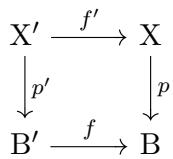
\includegraphics[keepaspectratio]{images/part001_94ec13ba.jpg}}

为一个笛卡尔方块。若映射 p 是分离的，则 p' 亦然。反之，若 p' 是分离的且 f 是普遍严格且满射的，则 p 是分离的。

考虑方块

\[
\begin{array}{c} \mathrm {X^ {\prime} \times_ {B^ {\prime}} X^ {\prime}} \xrightarrow {\varphi} \mathrm {X \times_ {B} X} \\ \Biggl \downarrow_ {q ^ {\prime}} \\ \mathrm {B^ {\prime} \xrightarrow {f} B} \end{array}
\]

其中映射 \(\varphi\) 由映射 \(f' \times f': X' \times X' \to X \times X\) 诱导。回顾 (I, p. 13, 例 1)，这个方块是笛卡尔的，并且有 \(\overline{\varphi}^1(\Delta_X) = \Delta_{X'}\) 。

若映射 p 是分离的，则集合 \(\Delta_{\mathrm{X}}\) 在 \(\mathrm{X} \times_{\mathrm{B}} \mathrm{X}\) 中是闭的；因此 \(\Delta_{\mathrm{X}'}\) 是 \(\mathrm{X}' \times_{\mathrm{B}'} \mathrm{X}'\) 的一个闭子集，这就证明了映射 \(p'\) 是分离的。

若映射 f 是满射的，则映射 \(\varphi\) 是满射的 (I, p. 10, cor.)；若 f 是普遍严格的，则 \(\varphi\) 是严格的 (I, p. 20, def. 6)。设映射 \(p'\) 是分离的。于是 \(\Delta_{\mathrm{X}'}\) 在 \(\mathrm{X}' \times_{\mathrm{B}'} \mathrm{X}'\) 中是闭的。由于 \(\Delta_{\mathrm{X}'} = \overline{\varphi}^{1}(\Delta_{\mathrm{X}})\) 且 \(\varphi\) 是满射且严格的，\(\Delta_{\mathrm{X}}\) 在 \(\mathrm{X} \times_{\mathrm{B}} \mathrm{X}\) 中是闭的，这就证明了映射 \(p\) 是分离的。

命题 5. --- 设 \(f: X \to Y\) 与 \(g: Y \to Z\) 为连续映射。设映射 \(g\) 是分离的且映射 \(g \circ f\) 是逆紧的。则映射 \(f\) 是逆紧的。

考虑下列笛卡尔方块：

\[
\begin{array}{c} \mathrm{X} \times_ {\mathrm{Z}} \mathrm{Y} \xrightarrow {\operatorname{pr} _ {2}} \mathrm{Y} \\ \Biggl \downarrow \operatorname{pr} _ {1} \\ \mathrm{X} \xrightarrow {g \circ f} \mathrm{Z}. \end{array}
\]

设 \(s \colon X \to X \times_{Z} Y\) 为映射 \(x \mapsto (x, f(x))\) 。它是 \(\mathrm{pr}_1 \colon X \times_{Z} Y \to X\) 的一个连续截面。由命题 4，映射 \(\mathrm{pr}_1\) 是分离的；由此推出映射 \(s\) 是逆紧的 (I, p. 27, prop. 3 与 TG, I, p. 72, prop. 2)。另一方面，映射 \(\mathrm{pr}_2\) 是逆紧的 (I, p. 17, prop. 8)。因此，映射 \(f\) （它等于 \(\mathrm{pr}_2 \circ s\) ）是逆紧的 (TG, I, p. 73, prop. 5)。

